\documentclass{article}

\usepackage{amsmath}
\usepackage{graphicx}
\usepackage{float}
\usepackage{fullpage}

% Default fixed font does not support bold face
\DeclareFixedFont{\ttb}{T1}{txtt}{bx}{n}{12} % for bold
\DeclareFixedFont{\ttm}{T1}{txtt}{m}{n}{12}  % for normal

% Custom colors
\usepackage{color}
\definecolor{deepblue}{rgb}{0,0,0.5}
\definecolor{deepred}{rgb}{0.6,0,0}
\definecolor{deepgreen}{rgb}{0,0.5,0}

\usepackage{listings}

% Python style for highlighting
\newcommand\pythonstyle{\lstset{
language=Python,
basicstyle=\ttm,
otherkeywords={self},             % Add keywords here
keywordstyle=\ttb\color{deepblue},
emph={MyClass,__init__},          % Custom highlighting
emphstyle=\ttb\color{deepred},    % Custom highlighting style
stringstyle=\color{deepgreen},
frame=tb,                         % Any extra options here
showstringspaces=false            % 
}}


% Python environment
\lstnewenvironment{python}[1][]
{
\pythonstyle
\lstset{#1}
}
{}

\title{Statistical Machine Learning: Assignment 1}
\author{Joris van Vugt, s4279859 \\ Luc Nies, s4136748}
\date{\today}

\begin{document}
\maketitle
\section*{Exercise 1}

\subsection*{1}
\begin{python}
def f(x):
    return 1 + np.sin(6 * (x - 2))

def noisy_f(x):
    noise = np.random.normal(0, 0.3)
    return noise + f(x)

# Generate data
D = [noisy_f(x) for x in np.linspace(0, 1, 10)]
T = [noisy_f(x) for x in np.linspace(0, 1, 100)]
\end{python}
\begin{figure}[H]
\centering
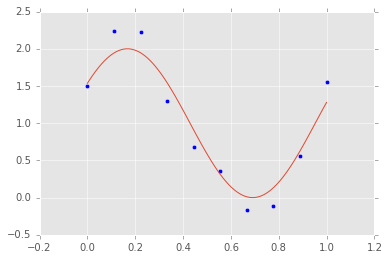
\includegraphics[width=.6\textwidth]{images/sin_d.png}
\caption{Plot of $f(x)$ and the 10 noisy observations in the training data}
\end{figure}

\subsection*{2}
\begin{python}
def pol_cur_fit(D, M):
    x = D[0, :]
    t = D[1, :]
    A = np.zeros((M, M))
    for i in range(M):
        for j in range(M):
            A[i, j] = np.sum(x ** (i+j))
    T = np.zeros(M)
    for i in range(M):
        T[i] = np.sum(t * x**i)
    w = np.linalg.solve(A, T)
    return w
\end{python}

\subsection*{3}
\begin{python}
def polynomial(X, w):
    return np.polyval(list(reversed(w)), X)

def RMSE(observed, target):
    error = 0.5 * np.sum((observed - target)**2)
    return np.sqrt(2*error / len(observed))
\end{python}
\begin{figure}[H]
\centering
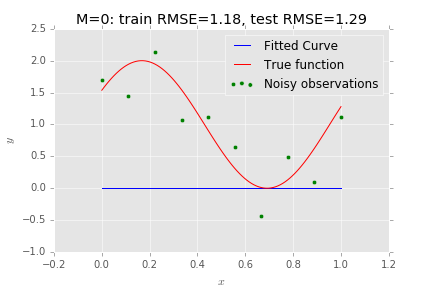
\includegraphics[width=.49\textwidth]{images/fit_m0_n_10.png}
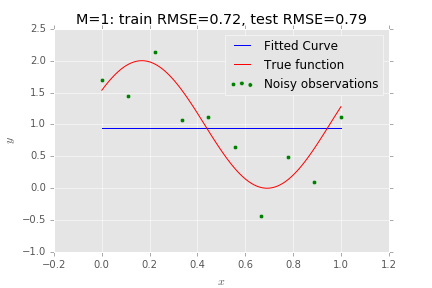
\includegraphics[width=.49\textwidth]{images/fit_m1_n_10.png}
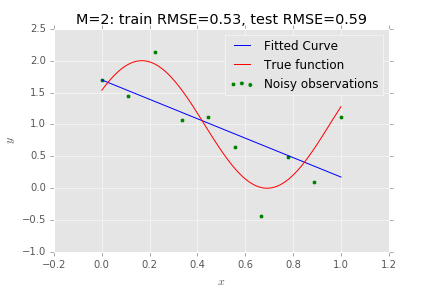
\includegraphics[width=.49\textwidth]{images/fit_m2_n_10.png}
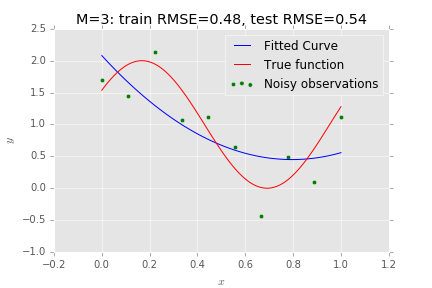
\includegraphics[width=.49\textwidth]{images/fit_m3_n_10.png}
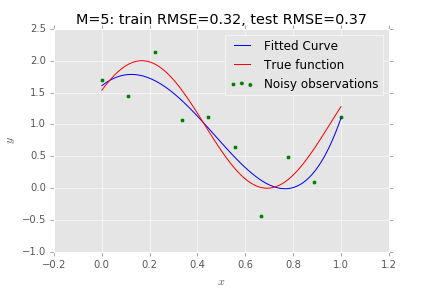
\includegraphics[width=.49\textwidth]{images/fit_m5_n_10.png}
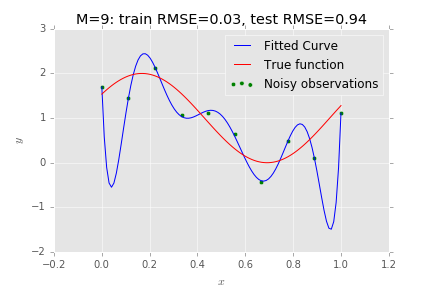
\includegraphics[width=.49\textwidth]{images/fit_m9_n_10.png}
\caption{Fitted curves for different values of M}
\end{figure}
When $M=2$, the polynomial is linear. From $M=4$ to $M=8$, the polynomial fits the underlying sine wave quite well. When $M=9$, the polynomial is clearly overfitted on the training data. This can also be concluded by comparing the root mean squared errors on the training and test sets.
\subsection*{4}
\begin{figure}[H]
\centering
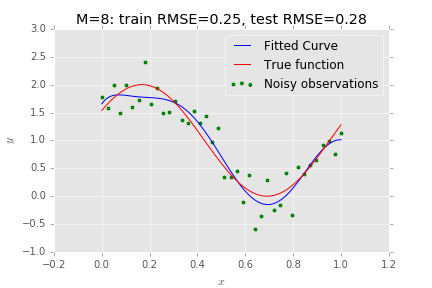
\includegraphics[width=0.6\textwidth]{images/fit_m8_n_40.png}
\caption{Fitted curve with $M=8$ and $N=40$}
\end{figure}
The fitted curves show less signs of overfitting overall and have lower errors. However for $M \geq 8$ there is still some overfitting to the noise, but since $N > M + 1$, the curve does not have enough degrees of freedom to fit all points exactly.
\subsection*{5}
\begin{table}[H]
\centering
\begin{tabular}{c | r | r}
$\textbf{w}$ & $\lambda=0$ & $\lambda=0.1$ \\
\hline
$w^*_0$ & 1.37 & 1.78 \\
$w^*_1$ & 61.59 & -1.19 \\
$w^*_2$ & -1022.49 & -1.29\\
$w^*_3$ & 7096.50 & -0.62 \\
$w^*_4$ & -25604.26 & -0.05 \\
$w^*_5$ & 51562.88 & 0.34 \\
$w^*_6$ & -58476.55 & 0.60 \\
$w^*_7$ & 34924.10 & 0.77 \\ 
$w^*_8$ & -8541.82 & 0.88 
\end{tabular}
\caption{Optimal weights for $M=9$ and $N=10$ with ($\lambda=0.1$)and without ($\lambda=0$) regularization}
\end{table}

The weigths with regularization are a lot smaller than the unregularized weights. There is also a smaller difference between the error on the test and the training set when using regularization.

\begin{figure}[H]
\centering
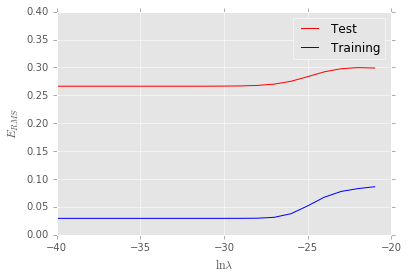
\includegraphics[width=0.6\textwidth]{images/effect_regularization.png}
\caption{The error on the training and test set versus the regularization strength}
\end{figure}
The reproduction of Figure 1.8 in Bishop looks slightly different for small values of $\ln \lambda$. We assume that the figure in Bishop is not on scale for $\ln \lambda < 35$ for educational purposes.

\section*{Exercise 2}
\subsection*{1}
\begin{figure}[H]
\centering
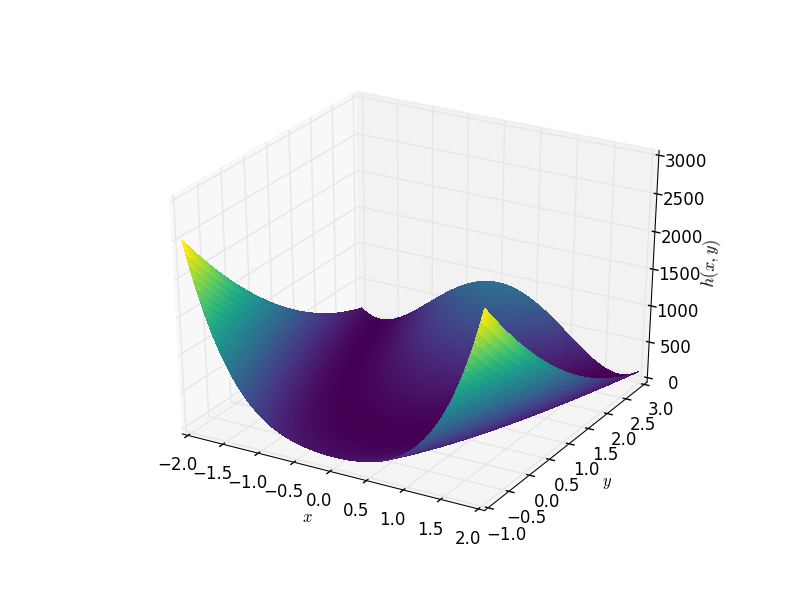
\includegraphics[width=.6\textwidth]{images/h.png}
\caption{Surface plot of $h(x, y)$}
\end{figure}
\begin{python}
def h(x, y):
    return 100 * (y - x**2)**2 + (1 - x)**2
\end{python}
We think that using gradient descent for this function will be slow, because there is a large `valley' (dark-blue area in the plot).
\end{document}